%!TEX root = ../thesis.tex
%******************************************************************************
\chapter{Background}\label{ch:background}
%******************************************************************************

This chapter further defines the context of the conducted research and introduces core concepts and terms that are used throughout the thesis. It starts with an introduction of batch and message-based processing. The terms latency and throughput are defined and their relationship is analyzed. 
The term \ac{SOA} is a briefly introduced, followed by a short description of \ac{ESB} middleware technology. Additionally, it describes \acp{EIP}, that can be used to improve the performance of messaging systems. The chapter describes performance issues of an \ac{SOA} middleware and discusses common approaches for performance optimizations of such a middleware.

\section{Batch Processing}\label{sec:batch_processing}
The traditional operation paradigm of a system for bulk data processing is batch processing (see Figure \ref{fig:batch_processing}). A batch processing system is an application that processes bulk data without user interaction. Input and output data is usually organised in records using a file- or database-based interface. In the case of a file-based interface, the application reads a record from the input file, processes it and writes the record to the output file.
\begin{figure}[htbp]
	\centering
	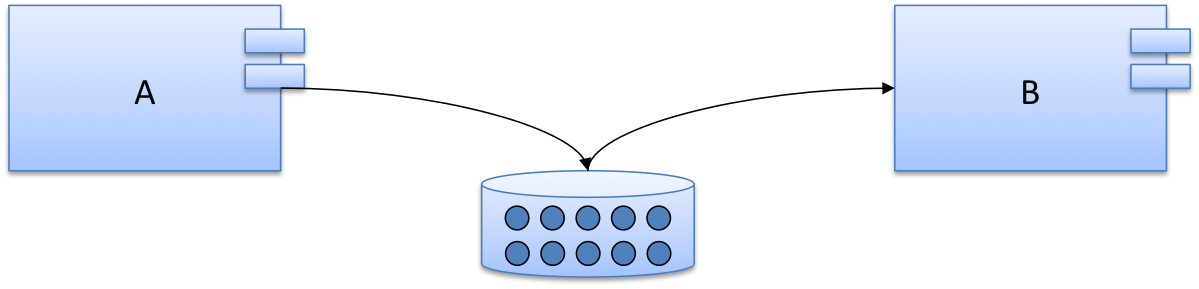
\includegraphics[width=\columnwidth]{batch}
	\caption{Batch processing}
	\label{fig:batch_processing}
\end{figure}

A batch processing system exhibits the following key characteristics:
\begin{itemize}
	\item \textbf{Bulk processing of data}\\
	A Batch processing system processes several gigabytes of data in a single run thus providing a high throughput. Multiple systems are running in parallel, controlled by a job scheduler to speed up processing. The data is usually partitioned and sorted by certain criteria for optimized processing. For example, if a batch only contains data for a specific product, the system can pre-load all necessary reference data from the database to speed up the processing.
	\item \textbf{No user interaction}\\
	There is no user interaction needed for the processing of data. It is impossible due to the amount of data being processed.
	\item \textbf{File- or database-based interfaces}\\
	Input data is read from the file system or a database. Output data is also written to files on the file system or a database. Files are transferred to the consuming systems through FTP by specific jobs.
	\item \textbf{Operation within a limited timeframe}\\
	A batch processing system often has to deliver its results in a limited timeframe due to \ac{SLA} with consuming systems. This timeframe is commonly called the batch window.
	\item \textbf{Offline handling of errors}\\
	Erroneous records are stored to a specific persistent memory (file or database) during operation and are processed afterwards.
\end{itemize}
Applications that are usually implemented as batch processing systems are billing systems for telecommunication companies used for mediating, rating and billing of call events.

\subsection{Integration Styles}
Batch processing systems use different styles to integrate with their outside environment or the integration of their subcomponents, with file-based and database-based integration being the most common. A combination of both styles is also possible.

\begin{itemize}
	\item \textbf{File transfer}\\
	With a file-based integration, the batch system or its subcomponents read the data from the input file, processes it and writes the output to the output file.
The file is transported to the next (sub-) system using \ac{FTP}, \ac{SCP} or other protocols for file transfer. The transfer is usually started by a specific job. Alternatively, a shared filesystem, such as \ac{NFS} can be used. The system also needs to be notified when new input data is ready for processing, for example by actively monitoring a certain folder or by getting notified from the previous system in the processing chain.
	\item \textbf{Shared database}\\
	The batch system or its subcomponents read and write the input and output data to a database, which is shared among all (sub-) systems. 
\end{itemize}

\subsection{Batch Performance Optimisations}

A batch-oriented system can be highly optimized for high throughput:

\begin{itemize}
	\item \textbf{Data formats}\\
	Using optimized data formats such as binary formats or \ac{CSV} data formats, that are optimized for reading and writing. Additionally, input and output data can be compressed to reduce data transfer times.
	\item \textbf{Database transactions}\\
	Database transactions introduce a major performance cost when processing large volumes of data. Batch processing system therefore minimize the amount of transactions by encapsulating a whole batch in one transaction, not every single record.
	\item \textbf{Database design and technologies}\\
	The database access can optimized by using pre-computed views especially designed for batch processing, such flattenend relations.
	Additionally, other database concepts than relational databases like No-SQL or in-memory databases can be used to further optimize the persistence layer.
	\item \textbf{Optimization depending on data semantics or technical properties}\\
	When data is processed in batches and is sorted accordingly to some business or technical rules, the processing algorithm can easily make assumptions about the data and optimize its processing. For example, when a batch only contains flat rate \ac{CDR} or \ac{CDR} of a specific product or customer segment, the corresponding reference data can be pre-loaded.
	\item \textbf{Caching}\\
	Often used data such as reference data, for example products and tariffs in case of a billing system, can also be cached in memory, prior to processing.
\end{itemize}

\subsection{Demarcation to Big Data}
Big Data is a term that generally describes large amounts of data, that is too big to process with traditional data processing applications, such as \ac{SQL}-based databases. In the context of \emph{Big Data}, a data processing application is defined as a system, that ``answers questions based on information that was acquired in the past'' (cf. \cite{Merz:2014aa}). These systems are commonly used in the realm of analytics to get better insights on the business. 

Technologies for implementing such as a system, like Apache Hadoop \citep{apachehadoop} are not considered for near-time processing of data, due to their high latency (cf. \cite{Merz:2014aa}).

\section{Message-based Processing}\label{sec:message_processing}
Messaging facilitates the integration of heterogeneous applications using asynchronous communication. Applications are communicating with each other by sending messages (see Figure \ref{fig:message_based_processing}). A messaging server or message-oriented middleware handles the asynchronous exchange of messages including an appropriate transaction control \citep{conrad2006enterprise}.

In the context of this thesis, messaging is a mean to implement single-event processing.

\begin{figure}[htbp]
	\centering
	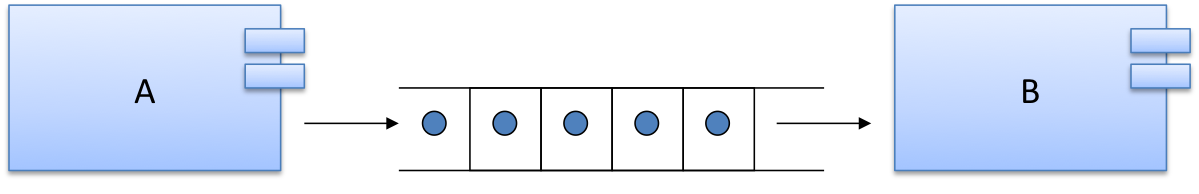
\includegraphics[width=\columnwidth]{esb}
	\caption{Message-based processing}
	\label{fig:message_based_processing}
\end{figure}

\cite{Hohpe:2003fk} describe the following basic messaging concepts:
\begin{itemize}
	\item \textbf{Channels}\\
	Messages are transmitted through a channel. A channel connects a message sender to a message receiver.
	\item \textbf{Messages}\\
	A message is packet of data that is transmitted through a channel. The message sender breaks the data into messages and sends them on a channel. The message receiver in turn reads the messages from the channel and extracts the data from them.
	\item \textbf{Pipes and Filters}\\
	A message may pass through several processing steps before it reaches its final destination. Multiple processing steps are chained together using a pipes and filters architecture.
	\item \textbf{Routing}\\
	A message may have to go through multiple channels before it reaches its destination. A message router acts as a filter and is capable of routing a message to the next channel or to another message router.
	\item \textbf{Transformation}\\
	A message can be transformed by a message translator if the message sender and receiver do not agree on the format for the same conceptual data.
	\item \textbf{Endpoints}\\
	A message endpoint is a software layer that connects arbitrary applications to the messaging system.
\end{itemize}

\subsection{Messaging Concepts}

There are two types of message channels (cf. \cite{Hohpe:2003fk}):

\begin{itemize}
	\item \textbf{Point To Point}\\
	A \emph{Point To Point} channel is used to send messages to only one receiver. The messaging system ensures that a message is consumed only once. A \emph{Point To Point} can also have multiple competing consumers, in this way, messages can be load-balanced among multiple consumers to scale the processing system. 
	\item \textbf{Publish-Subscribe}\\
	A \emph{Publish-Subscribe} channel is used to broadcast a message to multiple receivers. When a message is sent to input channel of the \emph{Publish-Subsriber} channel, the messaging system copies the message to multiple output channels, one chanel for each receiver. Each subscriber gets the message only once.
\end{itemize}

The adaptive middleware presented in this thesis only uses \emph{Point To Point} message channels with competing consumers.

Additionally, there are two important concepts for the transmission of messages (cf. \cite{Hohpe:2003fk}):

\begin{itemize}
	\item \textbf{Send and forget}\\
	The sending system sends the message to the message channel. The messaging system transmits the message in the background, the sender does not have to wait until the receiving system reads the message.
	\item \textbf{Store and forward}\\
	When the sending system sends the message to the message channel, the messaging system stores the message on the system of the sender and forwards it to the receiver by storing it to the receiving system. This can be repeated until the receiver receives the message.
\end{itemize}

In the context of this thesis, only \emph{Send and forget} is considered.
\\\\
Message-based systems are able to provide near-time processing of data due to their lower latency compared with batch processing systems. The advantage of a lower latency comes with a performance cost in regard to a lower throughput because of the additional overhead for each processed message. Every message needs amongst others to be serialised and deserialised, mapped between different protocols and routed to the appropriate receiving system. Section \ref{sec:ch02_performance_issues} contains a detailed discussion of performance issues of message-based service-oriented middleware.

\section{Latency vs. Throughput}\label{sec:ch2_latency_throughput}
Throughput and latency are performance metrics of a system. The following definitions of throughput and latency are used in this thesis:
\begin{itemize}
	\item \textbf{Maximum Throughput}\\
	The number of events the system is able to process in a fixed timeframe.
 	\item \textbf{Ent-to-end Latency}\\
	The period of time between the occurrence of an event and its processing. End-to-end latency refers to the total latency of a complete business process implemented by multiple subsystems. The remainder of this paper focusses on end-to-end latency using the general term latency as an abbreviation.
\end{itemize}
\subsubsection{Batch processing}
A business process, such as billing, implemented by a system using batch processing exhibits a high end-to-end latency. For example, consider the following billing system:
\begin{itemize}
	\item Customers are billed once per month
	\item Customers are partitioned in 30 billing groups
	\item The billing system processes 1 billing group per day, running 24h under full load.
\end{itemize}

In this case, the mean time for a call event to be billed by the billing system is $1/2$ month. That is, the mean end-to-end latency of this system is $1/2$ month.

\begin{figure}[h!]
	\centering
	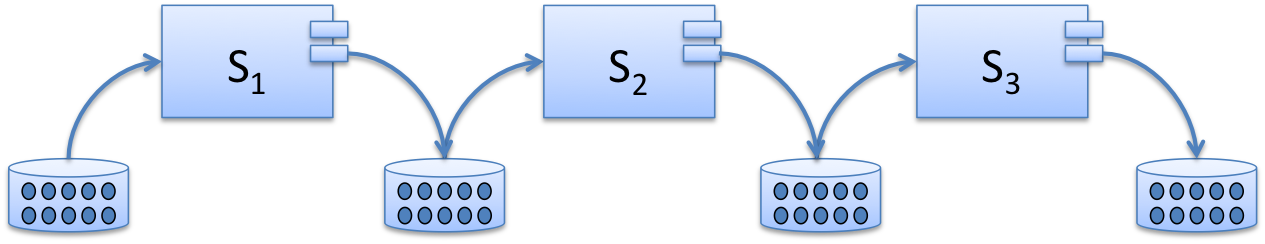
\includegraphics[width=\columnwidth]{latency_throughput1}
	\caption{Batch processing system comprised of three subsystems}
	\label{fig:batch_processing_latency}
\end{figure}

Assuming the system $S_{Batch}$ which is comprised of $N$ subsystems $S_1$, $S_2$, \ldots, $S_N$ (see Figure \ref{fig:batch_processing_latency} for an example with $N=3$):
\begin{displaymath}
S_{Batch} = \{S_1, S_2, \ldots, S_N\}
\end{displaymath}
The subsystem $S_i$ reads its input data from the database $DB_i$ in one chunk, processes it and writes the output to the database $DB_{i+1}$. When $S_i$ has finished the processing, the next subsystem $S_{i+1}$ reads the input data from $DB_{i+1}$, processes it and writes the output to $DB_{i+2}$, which in turn is read and processed from subsystem $S_{i+3}$ and so on.

The latency $L_{E_{S_{Batch}}}$ of a single event processed by the system $S_{Batch}$ is determined by the total processing time $PT_{S_{Batch}}$, which is the sum of the processing time $PT_i$ of each subsystem $S_i$:
\begin{displaymath}
L_{E_{S_{Batch}}} = PT_{S_{Batch}} = \sum_{i=1}^N PT_i
\end{displaymath}
where $N$ is the number of subsystems.

The processing time $PT_i$ of the subsystem $S_i$ is the sum of the processing time of each event $PT_{E_{j}}$ and the additional processing overhead $OH_i$, which includes the time spent for reading and writing the data, opening and closing transactions, etc:
\begin{displaymath}
PT_i = \left(\sum_{j=1}^M PT_{E_{j}}\right) + OH_i
\end{displaymath}
where $M$ is the number of events.

To allow for near-time processing, it is necessary to decrease the latency $L_{E_S}$ of a single event. This is can be achieved by using message-based processing instead of batch processing.

\subsubsection{Message-based processing}
The subsystem $S_i$ of a message-based system $S_{Message}$ reads a single event from its input message queue $MQ_i$, processes it and writes it to the output message queue $MQ_{i+1}$. As soon as the event is written to the message queue $MQ_{i+1}$, it is read by the subsystem $S_{i+1}$, which processes the event and writes to the message queue $MQ{i+2}$ and so on (see Figure \ref{fig:message_based_latency}).

The latency $L_{E_{S_{Message}}}$ of a single event processed by the system $S_{Message}$ is determined by the total processing time $PT_{E_{S_{Message}}}$ of this event, which is the sum of the processing time $PT_{E_i}$ and the processing overhead $OH_{E_{i}}$ for the event of each subsystem:
\begin{displaymath}
L_{E_{S_{Message}}} = PT_{E_{S_{Message}}} = \sum_{i+1}^N (PT_{E_i} + OH_{E_i})	
\end{displaymath}
where $N$ is the number of subsystems. Please note that the wait time of the event is assumed to be 0 for simplification.

The processing overhead $OH_{E_i}$ includes amongst others the time spent for unmarshalling and marshalling, protocol mapping and opening and closing transactions, which is done for every processed event.

\begin{figure}[h!]
	\centering
	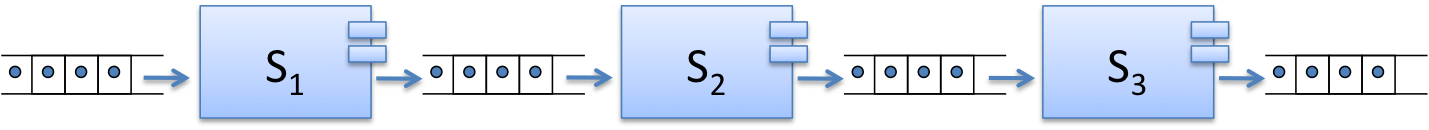
\includegraphics[width=\columnwidth]{latency_throughput2}
	\caption{Message-based system comprised of three subsystems}
	\label{fig:message_based_latency}
\end{figure}

Since the processing time $PT_{E_{S_{Message}}}$ of a single event is much shorter than the total processing time $PT_{S_{Batch}}$ of all events, the latency $L_{E_{S_{Message}}}$ of a single event using a message-based system is much smaller than the latency $L_{E_{S_{Batch}}}$ of a single event processed by a batch-processing system.
\begin{displaymath}
PT_{E_{S_{Message}}} < PT_{S_{Batch}} \Rightarrow L_{E_{S_{Message}}} < L_{E_{S_{Batch}}}
\end{displaymath}

Message-based processing adds an overhead to each processed event in contrast to batch processing, which adds a single overhead to each processing cycle. Hence, the accumulated total processing overhead $OH_{S_{Message}}$ of a message-based system $S_{Message}$ for processing $m$ events is larger than the total processing overhead of a batch processing system:
\begin{displaymath}
OH_{S_{Message}} = \sum_{i=1}^n OH_{E_i} * m > OH_{S_{Batch}} = \sum_{i=1}^n OH_i
\end{displaymath}
A message-based system, while having a lower end-to-end latency, is not able to process the same amount of events in the same time as a batch processing system and therefore cannot provide the same maximum throughput.

\begin{figure}[h!]
	\centering
	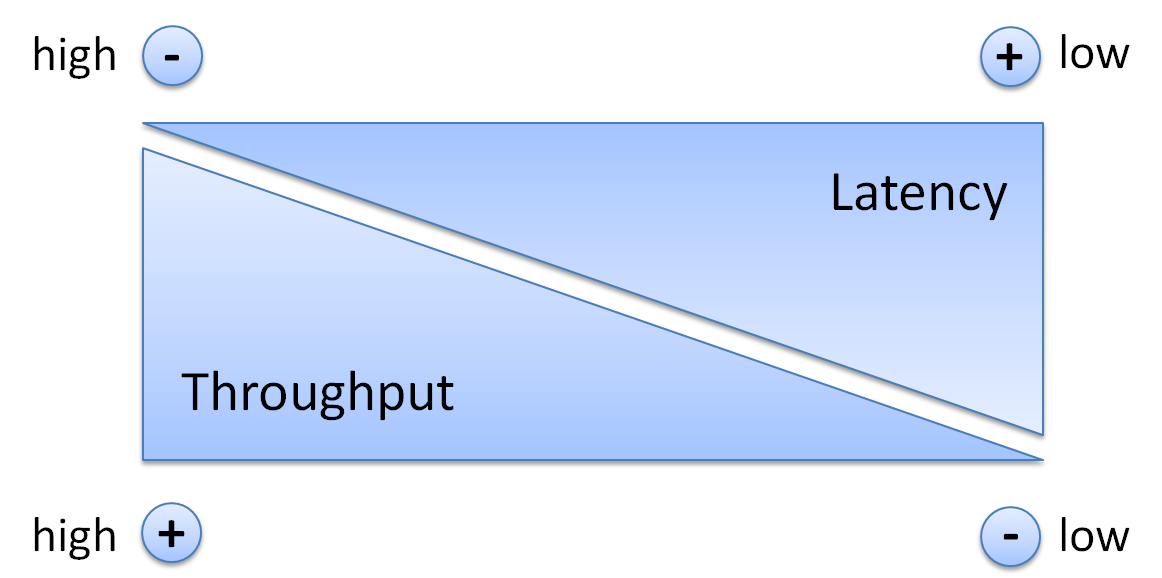
\includegraphics[width=\columnwidth]{latency_vs_throughput}
	\caption{Latency and throughput are opposed to each other}
	\label{fig:latency_vs_throughput}
\end{figure}

From this follows that latency and throughput are opposed to each other (see Figure \ref{fig:latency_vs_throughput}). High throughput, as provided by batch processing, leads to high latency, which impedes near-time processing. On the other hand, low latency, as provided by a message-based system, cannot provide the throughput needed for bulk data processing because of the additional overhead for each processed event.

\section{Service-Oriented Architecture}
\ac{SOA} is an architectural pattern to build application landscapes from single business components. These business components are loosely coupled by providing their functionality in form of services.  A service represents an abstract business view of the functionality and hides all implementation details of the component providing the service. The definition of a service acts as a contract between the service provider and the service consumer. Services are called using a unified mechanism, which provides a plattform independent connection of the business components while hiding all the technical details of the communication. The calling mechanism also includes the discovery of the appropriate service
\citep{Richter:2005ci}.

By separating the technical from the business aspects, SOA aims for a higher level of flexibility of enterprise applications.
\section{Enterprise Service Bus}
An \ac{ESB} is an integration platform that combines messaging, web services, data transformation and intelligent routing \citep{Schulte:2002mz}.
Table \ref{tab:char_esb} shows the main characteristics of an ESB \citep{Chappell:2004jo}.
\begin{table}[htbp]
	\centering
	\begin{tabular}{|p{0.3\textwidth}|p{0.6\textwidth}|}
		\hline
		Pervasiveness & An ESB supports multiple protocols and client technologies. It can span an entire organisation including its business partners. \\ \hline
		Highly distributed & An ESB integrates loosely coupled application components that form a highly distributed network. \\ \hline
		Selective deployment of integration components & The services of an ESB are independent of each other and can be separately deployed. \\ \hline
		Security and reliability & An ESB provides reliable messaging, transactional integrity and secure authentication. \\ \hline
		Orchestration and process flow & An ESB supports the orchestration of application components controlled by message metadata or an orchestration language like WS-BPEL. \\ \hline
		Autonomous yet federated managed environment & Different departments can still separately manage an ESB that spans the whole organisation. \\ \hline
		Incremental adoption & The adoption of an ESB can be incremental one project after another. \\ \hline
		XML support & XML is the native data format of an ESB. \\ \hline
		Real-time insight & An ESB provides real-time throughput of data by the use of its underlying message-oriented middleware and thus decreases latency. \\
		\hline
	\end{tabular}
	\caption{Main characteristics of an ESB \citep{Chappell:2004jo}}
	\label{tab:char_esb}
\end{table}
All application components and integration services that are connected to the ESB are viewed as abstract service endpoints. Abstract endpoints are logical abstractions of services that are plugged into the ESB and are all equal participants \citep{Chappell:2004jo}. An abstract endpoint can represent a whole application package such as a CRM or ERP system, a small web service or an integration service of the ESB such as a monitoring, logging or transformation service. As integration platform the ESB supports various types of connections for the service endpoints. These can be SOAP, HTTP, FTP, JMS or other programming APIs for C, C++, C\#, etc. It is often stated that ``if you can't bring the application to the bus, bring the bus to the application'' \citep{Chappell:2004jo}.

The backbone of the ESB is a message-oriented middleware (MOM), which provides an asynchronous, reliable and efficient transport of data between the service endpoints. The concrete protocol of the MOM, such as JMS, WS-Rel* or a proprietary protocol is thereby abstracted by the service endpoint. The ESB is thus a logical layer over the messaging middleware. The utilised protocol can also be varied by the ESB depending on the Quality of Service (QoS) requirements or deployment situations. Service endpoints can be orchestrated to process flows, which are mapped to concrete service invocations by the ESB.

The physical representation of a service endpoint is the service container. The service container is a remote process, which hosts the business or technical components that are connected through the bus. The set of all service containers therefore constitutes the logical ESB.

A service container provides the following interfaces \citep{Chappell:2004jo}:
\begin{itemize}
	\item \textbf{Service interface}\\
	The service interface provides an entry endpoint and exit endpoint to dispatch messages to and from the service.
	\item \textbf{Management interface}\\
	The management interface provides an entry endpoint for retrieving configuration data and an exit endpoint for sending, logging, event tracking and performance data.
\end{itemize}

\section{Enterprise Integration Patterns}
\label{sec:ch03_eip}

\acfp{EIP} describe a set of proven design patterns in the context of enterprise integration and messaging systems (cf. \cite{Hohpe:2003fk}). The adaptive middleware presented in this thesis is based on common \ac{EIP}, such as \emph{Aggregator} and \emph{Message Router}.

\subsection{Performance relevant \acp{EIP}}

The following \acp{EIP} are relevant for improving the performance of a message-based system and are used in the further course of the research presented in this thesis.

\subsubsection{Aggregator}
The \emph{Aggregator} is a stateful filter that correlates multiple received messages, aggregates them, and writes them as single message to its output channel (see Figure \ref{fig:ch02_aggregator}).

\begin{figure}[htbp]
	\centering
	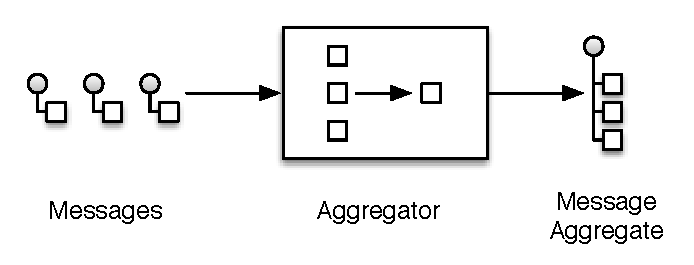
\includegraphics[width=0.7\textwidth]{ch02_aggregator}
	\caption{Aggregator \citep{Hohpe:2003fk}}
	\label{fig:ch02_aggregator}
\end{figure}

It is defined by the following properties:
\begin{itemize}
	\item \textbf{Correlation}\\
	Defines which messages should be correlated with each other.
	\item \textbf{Completeness Condition}\\
	Defines when a set of messages is ready to be written to the output channel.
	\item \textbf{Aggregation Algorithm}\\
	Defines how the received messages should be aggregated to a single message.
\end{itemize}

\cite{Hohpe:2003fk} describe the following most common strategies for completeness conditions:
\begin{itemize}
	\item \textbf{Wait for All}\\
	The aggregation is completed, when all messages are received. 
	\item \textbf{Timeout}\\
	The aggregation is completed when a defined timout occurs.
	\item \textbf{First Best}\\
	The \emph{Aggregator} waits until the first message is received.
	\item \textbf{Timeout with Override}\\
	The \emph{Aggregator} waits until a defined timeout occurs or until a message with a special content is received.
	\item \textbf{External Event}\\
	The aggregation is completed by an external event, for example the end of a business day.
\end{itemize}

Additionally, the authors describe the following strategies to aggregate messages into a single message \citep{Hohpe:2003fk}:
\begin{itemize}
	\item \textbf{Select the best answer}\\
	Only the ``best'' messages is passed to the output channel, all other messages are dismissed, for example the lowest bid for an item.
	\item \textbf{Condense data}\\
	The message data is aggregated into a single value, for example computing an average or a sum of a numerical value.
	\item \textbf{Collect data for later evaluation}\\
	Messages are simply combined into a single message. The decision how to aggregate can be done later by another component.
\end{itemize}

\subsubsection{Message Router}
The \emph{Message Router} reads messages from an input message channel and sends it to different output channels, depending on a set of conditions defined in the \emph{Message Router} (see Figure \ref{fig:ch02_message_router}).

\begin{figure}[htbp]
	\centering
	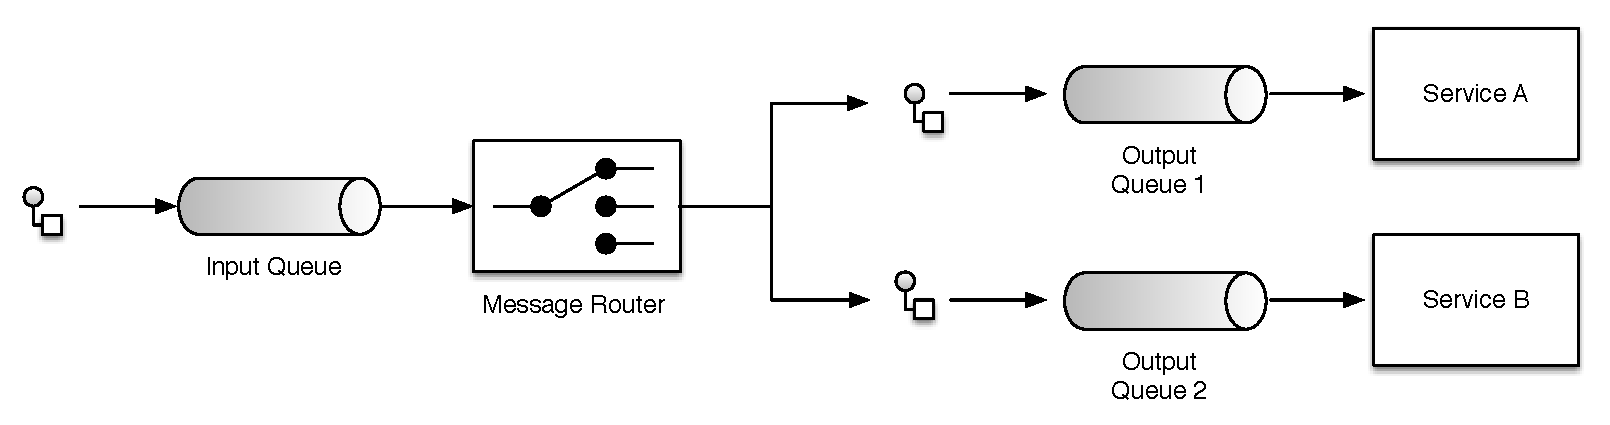
\includegraphics[width=\textwidth]{ch02_router}
	\caption{Message Router \citep{Hohpe:2003fk}}
	\label{fig:ch02_message_router}
\end{figure}

A \emph{Message Router} can implement different types of message routing:
\begin{itemize}
	\item \textbf{Content-based routing}\\
	The routing is based on the properties of a message, for example the message type or some business specific rules.
	\item \textbf{Context-based routing}\\
	The routing is based on conditions of the environment. This is used for example for load-balancing or failover strategies.
	\item \textbf{Dynamic routing}\\
	The routing is based on a dynamic rule base, which can be adapted at run-time.
\end{itemize}

\subsubsection{Content Filter}
A \emph{Content Filter} removes or simplifies unneeded data items from a message, only needed data items are left (see Figure \ref{fig:ch02_content_filter}).

\begin{figure}[htbp]
	\centering
	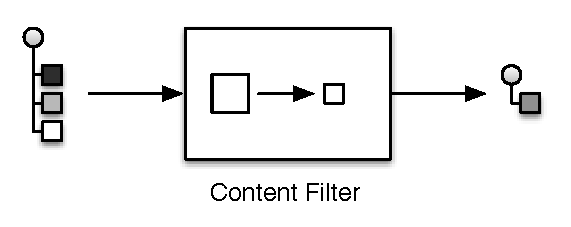
\includegraphics[width=0.6\textwidth]{ch02_content_filter}
	\caption{Content Filter \citep{Hohpe:2003fk}}
	\label{fig:ch02_content_filter}
\end{figure}

\subsubsection{Claim Check}

Since messaging adds an additional overhead to the processing of each message, for example by serializing and deserializing of data, it may be inefficient to send large volumes of data over a messaging system (cf. \cite{Hohpe:2003fk}). The \emph{Claim Check} pattern can used to mitigate this problem. It stores the payload of a message in a persistent data store and passes a unique identifier, the claim check, to the next components. Using this identifier, a component can retrieve the message payload from the data store and process the message (see Figure \ref{fig:ch02_claim_check}).

\begin{figure}[htbp]
	\centering
	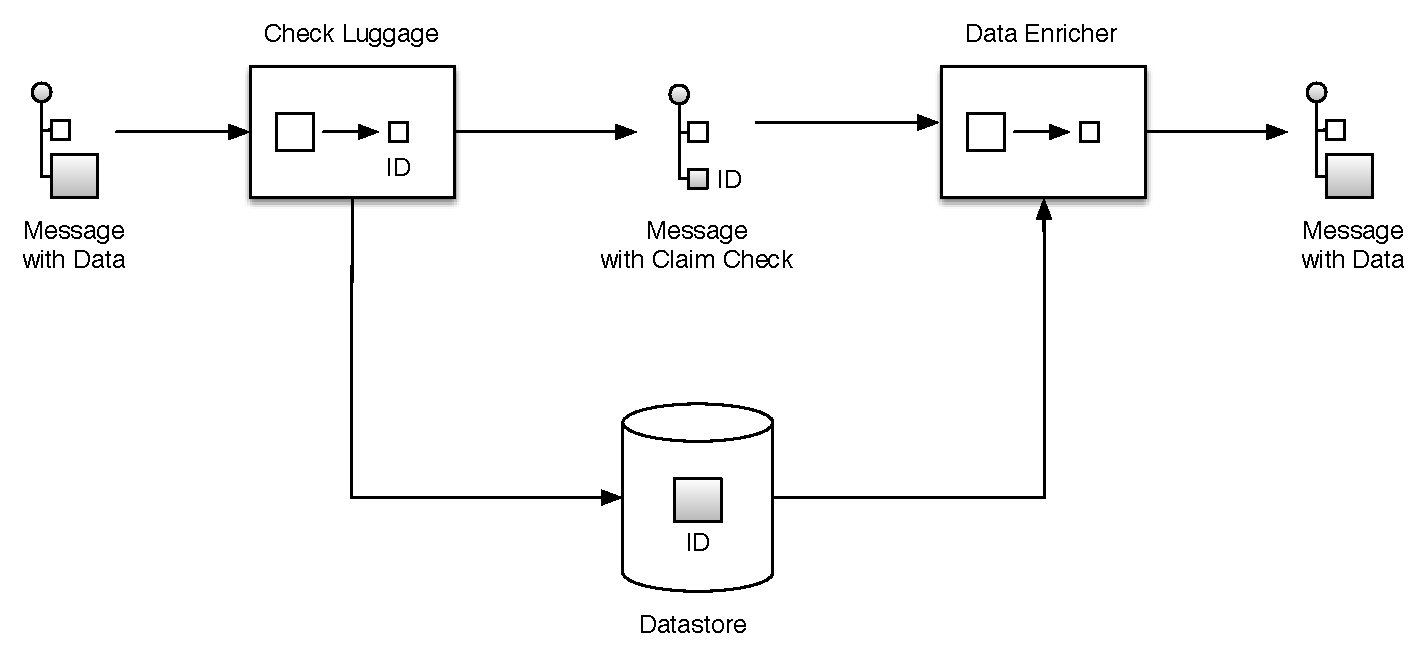
\includegraphics[width=\textwidth]{ch02_claim_check}
	\caption{Claim Check \citep{Hohpe:2003fk}}
	\label{fig:ch02_claim_check}
\end{figure}

\section{Performance Issues of Service-Oriented Middleware}
\label{sec:ch02_performance_issues}
This section describes the performance issues of an SOA middleware that inhibit their appropriateness for systems with high performance requirements.
\subsection{Distributed Architecture}
A system implemented according to the principles of SOA is a distributed system. Services are hosted on different locations belonging to different departments and even organizations. Hence, the performance drawbacks of a distributed system generally also apply to SOA. This includes the marshalling of the data that needs to be sent to the service provider by the service consumer, sending the data over the network and the unmarshalling of data by the service provider.
\subsection{Integration of Heterogeneous Technologies}
A main goal of introducing an SOA is to integrate applications implemented with heterogeneous technologies. This is achieved by using specific middleware and intermediate protocols for the communication. These protocols are typically based on XML, like SOAP \citep{soap:2007}. XML, as a very verbose language, adds a lot of meta-data to the actual payload of a message. The resulting request is about 10 to 20 times larger than the equivalent binary representation \citep{OBrien:2007fk}, which leads to a significant higher transmission time of the message. Processing these messages is also time-consuming, as they need to get parsed by a XML parser before the actual processing can occur.

The usage of a middleware like an Enterprise Service Bus (ESB) adds further performance costs. An ESB usually processes the messages during transferring. Among other things, this includes the mapping between different protocols used by service providers and service consumers, checking the correctness of the request format, adding message-level security and routing the request to the appropriate service provider (See, for example, \citet{Josuttis:2007fk} or \citet{Krafzig:2005zc}).
\subsection{Loose Coupling}
Another aspect of SOA that has an impact on performance is the utilisation of loose coupling. The aim of loose coupling is to increase the flexibility and maintainability of the application landscape by reducing the dependency of its components on each other. This denotes that service consumers shouldn't make any assumptions about the implementation of the services they use and vice versa. Services become interchangeable as long they implement the interface the client expects.

\citet{Engels:2008nr} consider two components A and B loosely coupled when the following constraints are satisfied:
\begin{itemize}
	\item \textbf{Knowlegde}\\
	Component A knows only as much as it is needed to use the operations offered by component B in a proper way. This includes the syntax and semantic of the interfaces and the structure of the transferred data.
	\item \textbf{Dependence on availability}\\
	Component A provides the implemented service even when component B is not available or the connection to component B is not available.
	\item \textbf{Trust}\\
	Component B does not rely on component A to comply with pre-conditions. Component A does not rely on component B to comply with post-conditions.
\end{itemize}

Coupling between services occurs on different levels. \citet{Krafzig:2005zc} describe the different levels of coupling that are leveraged in an \ac{SOA} (see Table \ref{table:ch02_coupling}).

\begin{table}[htpb]
	\centering
	\begin{tabularx}{\textwidth}{@{} X X X @{}}
		\caption{Levels of coupling}\label{table:ch02_coupling}\\
		\toprule
		\bfseries Level & \bfseries Tight Coupling & \bfseries Loose Coupling\\
		\midrule
		\bfseries Physical coupling & Direct physical link required & Physical intermediary\\
		\midrule
		\bfseries Communication style & Synchronous & Asynchronous\\
		\midrule
		\bfseries Type system & Strong type system & Weak type system\\
		\midrule
		\bfseries Interaction pattern & OO-style navigation of complex object trees & Data-centric, self-contained messages\\
		\midrule
		\bfseries Control of process logic & Central control of processing logic & Distributed logical components\\
		\midrule
		\bfseries Service discovery and binding & Statically bound services & Dynamically bound services\\
		\midrule
		\bfseries Platform dependencies & Strong OS and programming language dependencies & OS and programming languages independent\\
		\bottomrule
	\end{tabularx}
\end{table}

The gains in flexibility and maintainability of loose coupling are amongst others opposed by performance costs.

Service consumers and service providers are not bound to each other statically. Thus, the service consumer needs to determine the correct end point of the service provider during runtime. This can be done by looking up the correct service provider in a service repository either by the service consumer itself before making the call or by routing the message inside the ESB.  

Apart from very few basic data types, Service consumers and service providers do not share the same data model. It is therefore necessary to map data between the data model used by the service consumer and the data model used by the service provider.
\section{Current Approaches for Improving the Performance of an SOA Middleware}
This section describes current approaches to the performance issues introduced in the previous section.
\subsection{Hardware}
The obvious solution to improve the processing time of a service is the utilization of faster hardware and more bandwidth. SOA performance issues are often neglected by suggesting that faster hardware or more bandwidth will solve this problem. However, it is often not feasible to add faster or more hardware due to high cost pressure.
\subsection{Compression}
The usage of XML as an intermediate protocol for service calls has a negative impact on their transmission times over the network. The transmission time of service calls and responses can be decreased by compression. Simply compressing service calls and responses with gzip can do this. The World Wide Web Consortium (W3C) proposes a binary presentation of XML documents called binary XML \citep{EXI:2007} to achieve a more efficient transportation of XML over networks.

It must be pointed out that the utilisation of compression adds the additional costs of compressing and decompressing to the overall processing time of the service call.
\subsection{Service Granularity}
To reduce the communication overhead or the processing time of a service, the service granularity should be reconsidered.

\cite{Haesen:2008ve} distinguishes between two types of data granularity:
\begin{itemize}
	\item \textbf{Input data granularity}\\
	Data that is sent to a component
	\item \textbf{Output data granularity}\\
	Data that is returned by a component
\end{itemize}
The authors state that a coarse-grained data granularity reduces the communication overhead, since the number of network transfers is decreased.
``Especially in the case of Web services, this overhead is high since asynchronous messaging requires multiple queuing operations and numerous XML transformations''.

Coarse-grained services reduce the communication overhead by achieving more with a single service call and should be the favoured service design principle \citep{Hess:2006rs}. However, the processing time of a coarse-grained service can pose a problem to a service consumer that only needs a fracture of the data provided by the service. To reduce the processing time it could be considered in this case to add a finer grained service that provides only the needed data \citep{Josuttis:2007fk}. 

It should be noted that merging multiple services to form a more coarse-grained service or splitting a coarse-grained service into multiple services to solve performance problems specific to a single service consumer reduces the reusability of the services for other service consumers \citep{Josuttis:2007fk}.
\subsection{Degree of Loose Coupling}
The improvements in flexibility and maintainability gained by loose coupling are opposed by drawbacks on performance. Thus, it is crucial to find the appropriate degree of loose coupling. 

\citet{Hess:2006rs} introduce the concept of distance to determine an appropriate degree of coupling between components. The distance of components is comprised of the functional and technical distance. Components are functional distant if they share few functional similarities. Components are technical distant if they are of a different category. Categories classify different types of components like inventory components, process components, function components and interaction components.

Distant components trust each other in regard to the compliance of services levels to a lesser extent than near components do. The same applies to their common knowledge. Distant components share a lesser extent of knowledge of each other. Therefore, \citet{Hess:2006rs} argue that distant components should be coupled more loosely than close components.

The degree of loose coupling between components that have been identified to be performance bottlenecks should be reconsidered to find the appropriate trade-off between flexibility and performance. It can be acceptable in that case to decrease the flexibility in favour of a better performance. 

\subsection{Scaling}
Scalability describes the ``ability of a system to accommodate an increasing number of elements or objects, to process growing volumes of work gracefully, and/or to be susceptible to enlargement'' \citep{Bondi:2000jr}.

\cite{weinstock2006system} define scalability as:
\begin{enumerate}
	\item The ability to handle increased workload (without adding resources to a system).
	\item The ability to handle increased workload by repeatedly applying a cost-effective strategy for extending a system's capacity.
\end{enumerate}

\begin{itemize}
	\item \textbf{Horizontal scaling}\\
	Horizontal scaling involves adding more nodes to system, for example adding more servers to a distributed system and using a load-balancer to distribute the work between them.
	\item \textbf{Vertical scaling}\\
	Vertical scaling involves adding more resources to single node, such as additional \acp{CPU} or memory.
\end{itemize}

When a system is faced with infrequent load spikes, static scaling can lead to an overprovisioning of resources. The system is optimized to handle the load spikes, but is idle during the rest of the time.

\subsection{Dynamic Scaling}
A solution to prevent overprovisioning and to handle infrequent load spikes is to automatically instantiate additional server instances, as provided by current \ac{PaaS} offerings such as Amazon EC2 \citep{ec2_autoscaling} or Google App Engine \citep{google_cloud_autoscaling}. This is also called elasticity in the context of cloud computing (cf. \cite{Herbst:2013ug}).

While scaling is a common approach to improve the performance of a system, it also leads to additional operational and possible license costs. The solution presented in this thesis can be combined with these auto-scaling approaches to further increase the performance of the system.

\section{Summary}
Systems for bulk data processing are traditionally implemented using batch processing, for example billing systems for telecommunication providers. The performance requirements for such systems are high. They have to process millions of records in a fixed timeframe to comply with service level agreements.

Message-oriented middleware facilitates the integration of applications using asynchronous messages. Message-based systems are able to provide near-time processing of data due to their lower latency compared with batch processing systems. The advantage of a lower latency comes with a performance cost in regard to a lower throughput because of the additional overhead for each processed message. Every message needs amongst others to be serialised and deserialised, mapped between different protocols and routed to the appropriate receiving system. In the context of an \ac{SOA}, an Enterprise Service Bus is a common messaging middleware combining messaging, web services, data transformation and intelligent routing.

Common approaches to improve the performance of message-based systems try to reduce the transmission time by compressing messages, to adjust the service granularity to form more coarse-grained services or to adjust the degree of loose coupling to reduce the communication overhead. Scaling is a common approach to optimize the performance of of data processing system. Dynamic scaling is another solution to handle infrequent load spikes.

While these approaches generally improve the performance of mes\-sage-based systems, they are still not able provide the same throughput as that can be achieved with a batch processing system. Additionally, the current approaches are static and thus need to be considered at the design-time of the system. 

Systems are currently either optimized for bulk data processing or low latency. Alternatively, they use different components for batch and real-time processing. The proposed approached in this thesis, a middleware that is able to adapt its processing style fluently based on the current load of the system is a new approach which has not be considered so far by the state of art to the best of the author's knowlegde.